\documentclass[conference]{IEEEtran}

% -------------------------
% packages
% -------------------------
\usepackage[hidelinks]{hyperref}
\usepackage{amsmath,amssymb}
\usepackage{cite}
\usepackage{tabularx}
\usepackage{booktabs}
\usepackage{graphicx}
\usepackage{array}

% -------------------------
% table helpers
% -------------------------
\newcolumntype{Y}{>{\centering\arraybackslash}X}

% Look for figures in local artifacts or an Overleaf-style figures/ folder.
\graphicspath{{artifacts/paper/figures/}{figures/}}

% -------------------------
% title
% -------------------------
\title{Compute-Matched Depth Routing for Budget-Conditioned Anytime LLM Inference}
\author{Umberto Altieri}

\begin{document}
\maketitle

% ======================================================================
% abstract
% ======================================================================
\begin{abstract}
Fixed test-time budgets for large language models (LLMs) often allocate too much computation to easy examples and too little to hard ones. This paper studies depth routing for anytime inference when a model produces intermediate answers at increasing budgets. A budget-conditioned anytime model is trained by fine-tuning \texttt{Qwen2.5-Math-1.5B-Instruct} with QLoRA on GSM8K trajectories that contain four budgeted attempts and a self-reported confidence at each attempt (7,473 problems; 29,892 budget-labeled supervised fine-tuning examples). Lightweight stopping policies are then evaluated on the resulting 4-step trajectories without additional student weight updates; confidence-threshold routing additionally uses post-hoc per-split Platt calibration fitted on development data.

A compute-matched evaluation protocol is used: for each tier (B1--B4), adaptive routers are tuned to match the fixed-depth baseline's expected allocated-token compute, using a deterministic two-point mixture when exact matching is not attainable. On GSM8K test over three split seeds, confidence-threshold routing improves accuracy at B2 from 0.6603$\pm$0.0244 to 0.6937$\pm$0.0063 at similar mean allocated tokens (256 vs.\ 260), while stability-based routing improves accuracy at B3 from 0.6540$\pm$0.0311 to 0.6844$\pm$0.0305 (480 vs.\ 484). An oracle stopping reference reaches 0.8010$\pm$0.0259 at 272.9$\pm$15.9 tokens, indicating substantial headroom. Transfer to BoolQ without further fine-tuning is markedly weaker, and self-reported confidence is less effective than on GSM8K.
\end{abstract}

\begin{IEEEkeywords}
Test-time compute, anytime prediction, early stopping, routing, calibration, large language models
\end{IEEEkeywords}

% ======================================================================
\section{Introduction}
Reasoning-oriented LLMs often benefit from generating more tokens, for example under chain-of-thought prompting~\cite{wei2022cot}. Fixed inference budgets, however, are inefficient: easy examples may receive unnecessary computation, while difficult examples may still be under-served. A natural alternative is \emph{anytime inference}, in which a model emits intermediate answers under increasing budgets and a stopping policy decides when enough computation has been spent for a particular input.

This paper studies a simple version of that setting. A budget-conditioned student model is trained to produce an answer and a confidence value at four discrete budgets. Lightweight routers then decide whether to stop or continue based on the partial trajectory, without changing model weights at routing time.

A central empirical observation is that later budgets are not guaranteed to improve performance. On GSM8K, the trained adapter is stronger at intermediate checkpoints than at the largest budget (Section~\ref{sec:anytime-results}). Depth routing is therefore useful not only for reducing compute, but also for avoiding answer regressions caused by continued generation.

\paragraph{Contributions.}
\begin{itemize}
  \item A budget-conditioned anytime model is trained on GSM8K to emit both an answer and a self-reported confidence at four discrete budgets using automatically generated teacher trajectories.
  \item A compute-matched depth-routing protocol is formalized, including deterministic mixture policies that hit target expected token budgets without Monte Carlo variance.
  \item On GSM8K, simple confidence- and stability-based routers improve accuracy over fixed-depth baselines at matched compute in the intermediate budget regime.
  \item Transfer results on BoolQ show that confidence signals learned from math trajectories do not directly carry over to yes/no question answering without adaptation.
\end{itemize}

% ======================================================================
\section{Related Work}
\paragraph{Test-time compute and inference-time scaling.}
Several approaches improve reasoning by spending more computation at inference time, including longer deliberation, multiple samples, and self-consistency~\cite{wang2022selfconsistency}. The focus here is not sample aggregation, but per-example allocation and the decision of \emph{when to stop} under a fixed expected compute budget.

\paragraph{Anytime prediction and early exiting.}
Anytime prediction and adaptive computation have a long history. In deep networks, early-exit mechanisms reduce average compute by exiting when confidence is high~\cite{xin2020deebbert}. The present setting applies the same idea to LLM generation trajectories without architectural modifications to the backbone.

\paragraph{Confidence and calibration.}
Confidence estimates are central to selective prediction and abstention, while calibration methods aim to align confidence with empirical correctness~\cite{guo2017calibration,kadavath2022know}. The routing policies considered here use the model's self-reported \texttt{CONF: p} signal and optionally apply per-budget Platt calibration fitted on a development split.

% ======================================================================
\section{Method}
\subsection{Budget-Conditioned Anytime Inference}
A discrete budget index $t\in\{1,2,3,4\}$ is considered. For each input $x$, the anytime model is prompted at each budget $t$ and produces a response that includes (i) a final answer on a line prefixed by \texttt{\#\#\#\#} and (ii) a confidence score on a line prefixed by \texttt{CONF:}. For GSM8K, the final answer is numeric. For BoolQ, the output format constrains the final answer to \texttt{yes} or \texttt{no}.

\subsection{Trajectory Distillation on GSM8K}
Teacher trajectories for GSM8K are generated through an OpenAI Batch workflow using \texttt{gpt-4o-mini} as the default teacher model. The resulting training file contains 7,473 problems, each with four checkpoints. These trajectories are converted into supervised fine-tuning examples conditioned on the requested budget, yielding 29,892 training rows in total.

\subsection{Student Training}
The student model is \texttt{Qwen2.5-Math-1.5B-Instruct}, fine-tuned with QLoRA using 4-bit NF4 quantization, LoRA rank $r{=}16$, $\alpha{=}32$, dropout 0.05, target modules \texttt{q\_proj}, \texttt{k\_proj}, \texttt{v\_proj}, \texttt{o\_proj}, \texttt{gate\_proj}, \texttt{up\_proj}, and \texttt{down\_proj}, learning rate $2\times 10^{-4}$, one epoch, batch size 1, and gradient accumulation 16.

\subsection{Depth-Routing Policies}
Given a trajectory $\{(\hat{y}_t, \hat{p}_t)\}_{t=1}^4$, a router chooses a stop step $s$ and returns $\hat{y}_s$. The following policies are evaluated:
\begin{itemize}
  \item \textbf{Fixed:} stop at step $k$.
  \item \textbf{Confidence threshold:} stop at the first step with $\hat{p}_t \ge \tau$, otherwise continue to step 4.
  \item \textbf{Stability:} stop when the extracted answer remains unchanged for $m$ consecutive steps, subject to a minimum-step constraint.
  \item \textbf{Random matched:} match the confidence router's stopping histogram from the development set and report deterministic expected metrics.
  \item \textbf{Oracle reference:} stop at the earliest correct step, computed offline from the full trajectory.
\end{itemize}
When a step is missing a \texttt{CONF} value, the evaluation code defaults the confidence to 0.5.

\subsection{Compute-Matched Evaluation (Option-B)}
\label{sec:optionb}
Routers are evaluated under a compute-matched protocol. Compute tiers B1--B4 are defined by fixed-depth baselines with $k\in\{1,2,3,4\}$. For each tier and each seed, adaptive routers are tuned on a development split to match the fixed baseline's \emph{expected} mean token compute. The compute proxy is the cumulative sum of allocated per-step tokens. Under the default schedule, per-step budgets are $\{96,160,224,320\}$, which yields cumulative budgets $\{96,256,480,800\}$. If exact matching is not achievable with a single router setting, a deterministic two-point mixture is constructed between the nearest below-target and above-target settings, and expected metrics are reported analytically.

% ======================================================================
\section{Experimental Setup}
\paragraph{Datasets.}
Main results are reported on GSM8K~\cite{cobbe2021gsm8k} test (1,319 problems). Transfer results are reported on BoolQ~\cite{clark2019boolq} \emph{validation}. The canonical BoolQ paper artifact is \texttt{artifacts/router\_optionB\_boolq/paper\_table\_validation\_full\_per\_seed.csv}, which uses validation split labels consistently.

\paragraph{Splits and seeds.}
Router tuning uses three development/test partitions built with seeds $\{0,1,2\}$ and a test fraction of 0.2. Reported routing results are mean$\pm$std across these three seeds.

\paragraph{Calibration.}
Confidence-threshold routing uses per-seed Platt calibrators fitted on the corresponding development splits.

\paragraph{Evaluation metrics.}
Accuracy, mean allocated tokens, and mean stopping step are reported. The paper also examines the underlying anytime accuracies of the base model and the trained adapter.

% ======================================================================
\section{Results}

\subsection{Anytime Model Quality on GSM8K}
\label{sec:anytime-results}
Before routing, the quality of the underlying trajectories is measured. Table~\ref{tab:anytime_gsm8k} summarizes the unadapted base model and the trained adapter at each budget $t$ on GSM8K test.

\begin{table}[t]
\centering
\small
\setlength{\tabcolsep}{3.5pt}
\renewcommand{\arraystretch}{1.1}
\begin{tabular}{lcccc}
\toprule
Model & Acc@1 & Acc@2 & Acc@3 & Acc@4 \\
\midrule
Base model & 0.0281 & 0.0751 & 0.2487 & 0.5595 \\
Trained adapter & 0.6505 & 0.7096 & 0.7096 & 0.6869 \\
\bottomrule
\end{tabular}
\caption{Anytime accuracy on GSM8K test at each budget $t$ under strict answer matching.}
\label{tab:anytime_gsm8k}
\end{table}

Two properties are important for routing. First, the trained adapter is much stronger than the base model at low budgets. Second, accuracy is not monotone in budget: Acc@2 and Acc@3 exceed Acc@4. This non-monotonicity creates room for routing to improve both efficiency and accuracy. These anytime metrics are computed from the prediction bundle used for paper calibration/coverage figures, while the routing table in Table~\ref{tab:main_results_allbudgets} is sourced from the canonical Option-B router CSVs; the repository does not claim they are the same row-identical bundle.

\subsection{Compute-Matched Routing on GSM8K}
Table~\ref{tab:main_results_allbudgets} reports compute-matched routing results on GSM8K test using the Option-B protocol from Section~\ref{sec:optionb}.

\begin{table*}[t]
\centering
\small
\setlength{\tabcolsep}{3pt}
\renewcommand{\arraystretch}{1.1}
\begin{tabularx}{\textwidth}{lYYYY}
\toprule
Policy (test, mean$\pm$std over seeds, sample std) & B1 & B2 & B3 & B4 \\
\midrule
Fixed & 0.6464$\pm$0.0274 (96$\pm$0, 1.00$\pm$0.00) & 0.6603$\pm$0.0244 (256$\pm$0, 2.00$\pm$0.00) & 0.6540$\pm$0.0311 (480$\pm$0, 3.00$\pm$0.00) & 0.6527$\pm$0.0209 (800$\pm$0, 4.00$\pm$0.00) \\
\addlinespace
Confidence & 0.6464$\pm$0.0274 (96$\pm$0, 1.00$\pm$0.00) & 0.6937$\pm$0.0063 (260$\pm$19, 1.80$\pm$0.07) & 0.6654$\pm$0.0201 (483$\pm$17, 2.82$\pm$0.07) & 0.6527$\pm$0.0209 (800$\pm$0, 4.00$\pm$0.00) \\
Random (matched) & 0.6464$\pm$0.0274 (96$\pm$0, 1.00$\pm$0.00) & 0.6494$\pm$0.0224 (256$\pm$0, 1.78$\pm$0.08) & 0.6561$\pm$0.0217 (480$\pm$0, 2.81$\pm$0.02) & 0.6527$\pm$0.0209 (800$\pm$0, 4.00$\pm$0.00) \\
Stability (tuned) & 0.6464$\pm$0.0274 (96$\pm$0, 1.00$\pm$0.00) & 0.6710$\pm$0.0251 (258$\pm$5, 1.83$\pm$0.02) & 0.6844$\pm$0.0305 (484$\pm$10, 2.93$\pm$0.03) & 0.6527$\pm$0.0209 (800$\pm$0, 4.00$\pm$0.00) \\
Oracle & 0.8010$\pm$0.0259 (273$\pm$20, 1.80$\pm$0.08) & 0.8010$\pm$0.0259 (273$\pm$20, 1.80$\pm$0.08) & 0.8010$\pm$0.0259 (273$\pm$20, 1.80$\pm$0.08) & 0.8010$\pm$0.0259 (273$\pm$20, 1.80$\pm$0.08) \\
\bottomrule
\end{tabularx}
\caption{Test performance across compute tiers (accuracy; mean tokens and mean steps in parentheses). Values are mean$\pm$std over three split seeds (sample std).}
\label{tab:main_results_allbudgets}
\end{table*}


At B2, confidence routing yields the largest gain over fixed depth (0.6937 vs.\ 0.6603) at nearly identical compute. At B3, stability routing performs best among the non-oracle policies (0.6844 vs.\ 0.6540). The random-matched baseline remains close to fixed depth, suggesting that the gains arise from using trajectory information rather than merely changing the stopping histogram. The oracle reference indicates large remaining headroom: many examples are solvable earlier than B4, but the available signals do not yet identify those cases reliably.

\subsection{Transfer to BoolQ}
Table~\ref{tab:router_boolq} reports compute-matched transfer results on BoolQ validation using the same GSM8K-trained anytime model and the same router family, with router tuning performed on BoolQ development splits and no additional model fine-tuning.

\begin{table*}[t]
\centering
\small
\setlength{\tabcolsep}{3pt}
\renewcommand{\arraystretch}{1.1}
\begin{tabularx}{\textwidth}{lYYYY}
\toprule
Policy (validation, mean$\pm$std over seeds) & B1 & B2 & B3 & B4 \\
\midrule
Fixed & 0.1200$\pm$0.0173 (96$\pm$0, 1.00$\pm$0.00) & 0.2633$\pm$0.0751 (256$\pm$0, 2.00$\pm$0.00) & 0.4367$\pm$0.0493 (480$\pm$0, 3.00$\pm$0.00) & 0.4833$\pm$0.0208 (800$\pm$0, 4.00$\pm$0.00) \\
\addlinespace
Confidence & 0.1200$\pm$0.0173 (96$\pm$0, 1.00$\pm$0.00) & 0.2026$\pm$0.0129 (256$\pm$0, 1.68$\pm$0.00) & 0.3182$\pm$0.0119 (480$\pm$0, 2.64$\pm$0.00) & 0.4833$\pm$0.0208 (800$\pm$0, 4.00$\pm$0.00) \\
Random (matched) & 0.1200$\pm$0.0173 (96$\pm$0, 1.00$\pm$0.00) & 0.2026$\pm$0.0129 (256$\pm$0, 1.68$\pm$0.00) & 0.3182$\pm$0.0119 (480$\pm$0, 2.64$\pm$0.00) & 0.4833$\pm$0.0208 (800$\pm$0, 4.00$\pm$0.00) \\
Stability (tuned) & 0.1200$\pm$0.0173 (96$\pm$0, 1.00$\pm$0.00) & 0.2519$\pm$0.0188 (256$\pm$0, 1.83$\pm$0.00) & 0.3934$\pm$0.0536 (477$\pm$4, 2.83$\pm$0.01) & 0.4833$\pm$0.0208 (800$\pm$0, 4.00$\pm$0.00) \\
Oracle & 0.6133$\pm$0.0503 (554$\pm$35, 3.08$\pm$0.13) & -- & -- & -- \\
\bottomrule
\end{tabularx}
\caption{Validation performance across compute tiers (accuracy; mean tokens and mean steps in parentheses). Values are mean$\pm$std over three split seeds.}
\label{tab:router_boolq}
\end{table*}


In this transfer setting, confidence routing underperforms fixed depth at B2 and B3, while stability remains closer to the fixed-depth baseline. This pattern suggests that the confidence signal learned from GSM8K-style mathematical reasoning does not directly transfer to yes/no question answering.

\subsection{Accuracy--Compute Visualization}
Figure~\ref{fig:pareto} shows the accuracy--compute trade-off for the routing policies on GSM8K.

\begin{figure}[t]
\centering
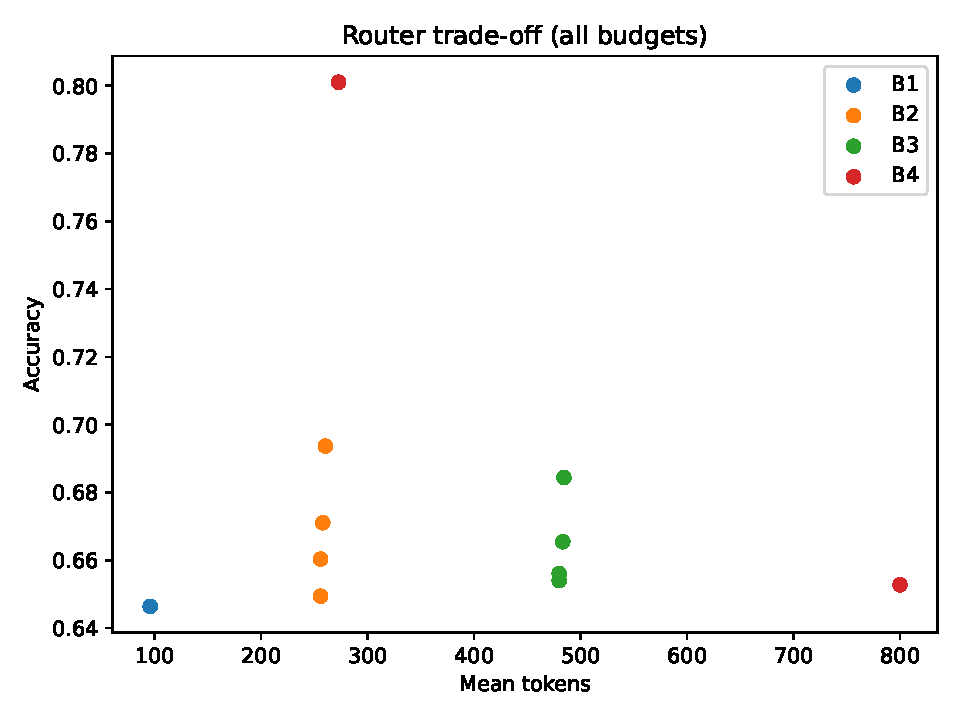
\includegraphics[width=0.98\linewidth]{router_pareto_all.pdf}
\caption{Accuracy versus mean allocated tokens for routing policies on GSM8K.}
\label{fig:pareto}
\end{figure}

% ======================================================================
\section{Discussion and Limitations}
\paragraph{Why stability helps at B3.}
Stability uses answer agreement across budgets, which becomes informative once trajectories are long enough to exhibit answer flips. On GSM8K, that behavior aligns with the observed non-monotonicity across budgets for the trained adapter.

\paragraph{Confidence transfer is fragile.}
On BoolQ, confidence-threshold routing is substantially worse than fixed depth at intermediate tiers. This is consistent with confidence being task- and format-dependent. Better transfer may require task-specific calibration, alternative uncertainty signals such as log-probability margins, or training trajectories that cover yes/no tasks directly.

\paragraph{Allocated versus realized compute.}
The compute-matched protocol uses allocated tokens (\texttt{max\_new\_tokens}) as a stable proxy for inference cost. Actual generated tokens are also available in the evaluation pipeline, but they are not used when constructing routing costs. Conclusions should therefore be interpreted as matching \emph{allocated} rather than realized compute.

\paragraph{Scope limitations.}
The empirical study uses a single 1.5B backbone, four discrete budgets, and three split seeds. Reported variability is split-seed variability from router dev/test partitioning only, and does not include retraining/model-seed variance for the student or router feature pipeline. The transfer experiment also omits target-task fine-tuning and is only partially reproducible from this snapshot because some BoolQ-side inputs are Git LFS/externally dependent. Broader conclusions about scaling, architecture dependence, and cross-domain robustness will require a larger experimental sweep.

% ======================================================================
\section{Reproducibility}
The experimental pipeline is script-driven and partially reproducible from the shipped repository. Tables and figures can be regenerated from bundled prediction/router artifacts, and paper claims are artifact-level claims tied to those canonical files rather than a full raw-to-paper rerun guarantee. Split-seed router variability can be recomputed from bundled manifests, while model-seed retraining variability is not evaluated in the released artifact. Full end-to-end regeneration (including trajectory generation and some evaluation splits such as BoolQ transfer inputs) depends on external datasets, model checkpoints, and Git LFS objects not bundled directly in this snapshot.

% ======================================================================
\section{Conclusion}
Budget-conditioned anytime inference provides a useful setting for studying adaptive test-time compute in LLMs. Under matched expected compute, lightweight depth routers improve intermediate-budget performance on GSM8K relative to fixed-depth baselines. Confidence-threshold routing is strongest at B2, while stability-based routing is strongest at B3. Transfer to BoolQ without further fine-tuning is substantially less favorable, especially for confidence-based stopping, which suggests that confidence signals learned on math reasoning do not directly generalize across tasks. The oracle reference indicates considerable room for stronger stopping criteria.

% ======================================================================
\begin{thebibliography}{00}

\bibitem{wei2022cot}
J.~Wei \emph{et~al.}, ``Chain-of-Thought Prompting Elicits Reasoning in Large Language Models,'' \emph{arXiv:2201.11903}, 2022.

\bibitem{wang2022selfconsistency}
X.~Wang \emph{et~al.}, ``Self-Consistency Improves Chain of Thought Reasoning in Language Models,'' \emph{arXiv:2203.11171}, 2022.

\bibitem{zhou2022leasttomost}
D.~Zhou \emph{et~al.}, ``Least-to-Most Prompting Enables Complex Reasoning in Large Language Models,'' \emph{arXiv:2205.10625}, 2022.

\bibitem{xin2020deebbert}
J.~Xin \emph{et~al.}, ``DeeBERT: Dynamic Early Exiting for Accelerating BERT Inference,'' in \emph{Proceedings of the 58th Annual Meeting of the Association for Computational Linguistics (ACL)}, 2020.

\bibitem{guo2017calibration}
C.~Guo, G.~Pleiss, Y.~Sun, and K.~Q.~Weinberger, ``On Calibration of Modern Neural Networks,'' in \emph{Proceedings of the 34th International Conference on Machine Learning (ICML)}, 2017.

\bibitem{kadavath2022know}
S.~Kadavath \emph{et~al.}, ``Language Models (Mostly) Know What They Know,'' \emph{arXiv:2207.05221}, 2022.

\bibitem{cobbe2021gsm8k}
K.~Cobbe \emph{et~al.}, ``Training Verifiers to Solve Math Word Problems,'' \emph{arXiv:2110.14168}, 2021.

\bibitem{clark2019boolq}
C.~Clark \emph{et~al.}, ``BoolQ: Exploring the Surprising Difficulty of Natural Yes/No Questions,'' \emph{arXiv:1905.10044}, 2019.

\end{thebibliography}

\end{document}
